\begin{figure}[h]
	\centering
	\missingfigure{Verteilungsdiagramm}		
	\caption{Verteilungsdiagramm}
	\label{fig:verteilungsdiagramm}
\end{figure}

\begin{tcolorbox}
	Das zukünftige Deployment des Systems wird mittels einem Verteilungsdiagramm modelliert.
	Weiterhin sollten wichtige oder eventuell undeutliche Zusammenhänge (z.B. warum Schnittstelle X genutzt wird) in einem Fließtext beschrieben werden.
\end{tcolorbox}

\begin{figure}[H]
	\centering
	\caption{Verteilungsdiagramm}
	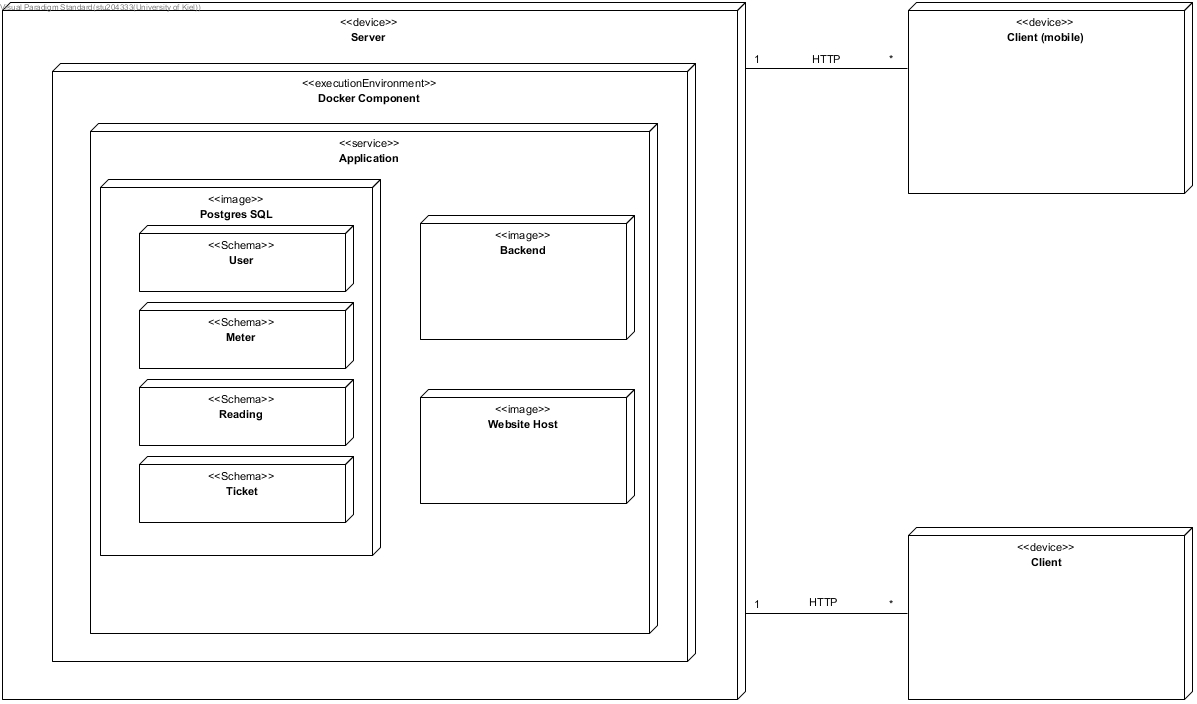
\includegraphics[width=16cm]{img/diagrams/DeploymentDiagram}
\end{figure}

Im Allgemeinen läuft die gesamte Software auf dem selben Server. Durch Docker werden einzelne Komponenten aber in unterschiedlichen Containern laufen.\\
So läuft in einem Container die Software für das Backend, die über eine REST-API mit dem Frontend kommuniziert. Die Web und App Anwendungen können dann HTTP Anfragen an das Backend stellen.\\
Ein weiterer Container beinhaltet die SQL-Datenbank. Diese beinhaltet Schemata für Nutzer, Zähler, Zählerstände und Tickets.
